\documentclass[11pt,a4paper]{article}

\usepackage[utf8]{vietnam}
\usepackage{amsmath,amssymb,amsthm}
\usepackage{graphicx}
\usepackage{hyperref}
\usepackage{geometry}
\usepackage{listings}
\usepackage{xcolor}
\usepackage{booktabs}
\usepackage{tabularx}
\usepackage{algorithm}
\usepackage{algpseudocode}
\usepackage{tikz}
\usetikzlibrary{arrows,positioning}

\geometry{margin=2.5cm}

\definecolor{codeblue}{RGB}{0,102,204}
\definecolor{codegray}{RGB}{128,128,128}

\lstdefinestyle{python}{
    language=Python,
    basicstyle=\footnotesize\ttfamily,
    keywordstyle=\color{codeblue},
    commentstyle=\color{codegray},
    numbers=left,
    numberstyle=\tiny,
    frame=single,
    breaklines=true,
    tabsize=4
}

\theoremstyle{definition}
\newtheorem{definition}{Definition}[section]

\title{\textbf{CRP-RL: Scale-diverse Deep Reinforcement Learning \\ for the Container Retrieval Problem}\\[4pt]
\large Tài liệu phương pháp và hướng dẫn Repository}
\author{Nghiên cứu sinh -- AI/ML/DL/Optimization}
\date{\today}

\begin{document}
\maketitle
\tableofcontents
\newpage

\section{Giới thiệu}

Bài toán \textbf{Container Retrieval Problem (CRP)} là một bài toán tối ưu hóa quan trọng trong lĩnh vực quản lý cảng container. Mục tiêu là thu hồi các container từ bãi xếp chồng theo một thứ tự nhất định, trong khi tối thiểu hóa tổng thời gian làm việc bao gồm thời gian di chuyển, thời gian xử lý và thời gian phạt.

Dự án \texttt{CRP-RL} (Container Retrieval Problem -- Reinforcement Learning) là hiện thực hóa của bài báo:
\begin{quote}
    Woo-Jin Shin, Inguk Choi, Sang-Hyun Cho, Hyun-Jung Kim. \\
    \textit{``Learning to Retrieve Containers: A Scale-diverse Deep Reinforcement Learning Approach for the Container Retrieval Problem.''} \\
    Transportation Research Part C: Emerging Technologies, 2026. \\
    DOI: \href{https://doi.org/10.1016/j.trc.2025.105496}{10.1016/j.trc.2025.105496}
\end{quote}

\subsection{Đóng góp chính}

\begin{enumerate}
    \item \textbf{Phương pháp DRL scale-diverse} — sử dụng mạng Transformer policy được huấn luyện với REINFORCE + baseline đề xuất, có khả năng tổng quát hóa trên nhiều kích thước bãi container khác nhau (1--30 bays).
    \item \textbf{Zero-shot multi-crane transfer} — áp dụng mô hình đơn crane sang môi trường nhiều crane mà không cần huấn luyện lại.
    \item \textbf{Lower bound cho M-CRP} — chặn dưới hình thức cho bài toán nhiều crane (Theorem 3).
    \item \textbf{Đánh giá toàn diện} — so sánh với các heuristic kinh điển (Lin2015, Kim2016, Leveling), GP-evolved rules và search-based methods.
\end{enumerate}

\subsection{Bài toán CRP}

\begin{definition}[Container Retrieval Problem]
Cho một bãi container gồm $B$ bays, $R$ rows, $T$ tiers và tập container $\mathcal{C}$ cần thu hồi theo thứ tự $\sigma = (\sigma_1, \sigma_2, \dots, \sigma_n)$. 
Mục tiêu là tìm một chuỗi hành động relocations để thu hồi toàn bộ container sao cho tổng thời gian làm việc:
\begin{equation}
    \text{TotalCost} = \sum (\text{travel\_time} + \text{handling\_time} + \text{penalty\_time})
\end{equation}
là nhỏ nhất.
\end{definition}

\newpage

\section{Phương pháp đề xuất}

\subsection{Tổng quan kiến trúc}

\begin{figure}[h!]
    \centering
    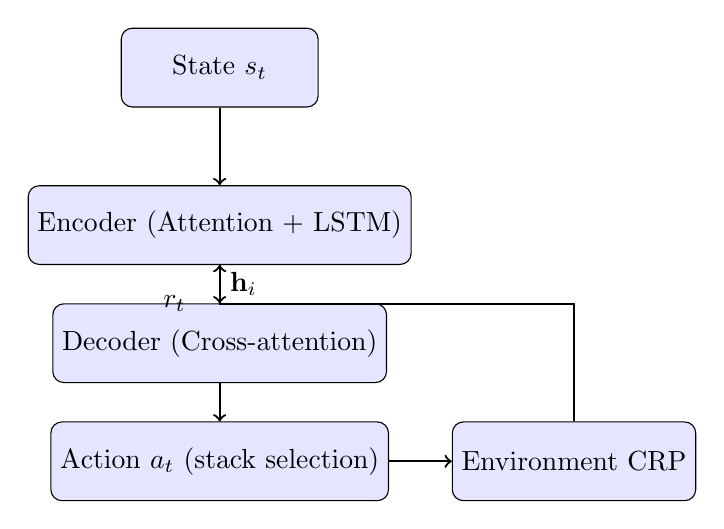
\begin{tikzpicture}[node distance=1.5cm, auto]
        \tikzstyle{block} = [rectangle, draw, rounded corners, minimum width=2.5cm, minimum height=1cm, text centered, fill=blue!10]
        \tikzstyle{arrow} = [->, thick]

        \node (input) [block] {State $s_t$};
        \node (encoder) [block, below of=input, yshift=-0.5cm] {Encoder (Attention + LSTM)};
        \node (decoder) [block, below of=encoder] {Decoder (Cross-attention)};
        \node (action) [block, below of=decoder] {Action $a_t$ (stack selection)};
        \node (env) [block, right of=action, xshift=3cm] {Environment CRP};

        \draw[arrow] (input) -- (encoder);
        \draw[arrow] (encoder) -- node[right] {$\mathbf{h}_i$} (decoder);
        \draw[arrow] (decoder) -- (action);
        \draw[arrow] (action) -- (env);
        \draw[arrow] (env) -- ++(0, 2cm) -| node[left, xshift=-0.3cm] {$r_t$} (encoder);
    \end{tikzpicture}
    \caption{Kiến trúc tổng quan của policy network.}
    \label{fig:architecture}
\end{figure}

\subsection{Encoder}

Encoder nhận đầu vào là trạng thái bãi container và xuất ra embedding cho mỗi stack.

\subsubsection{Expert Features}

Với mỗi stack $i$, ta trích xuất vector đặc trưng gồm:
\begin{itemize}
    \item \texttt{min\_due\_date}: priority nhỏ nhất trong stack
    \item \texttt{top\_priority}: priority của container trên cùng
    \item \texttt{well\_located}: cờ chỉ vị trí tốt (container đúng thứ tự)
    \item \texttt{height}: số container trong stack
    \item \texttt{row\_pos}, \texttt{bay\_pos}: vị trí row/bay
    \item \texttt{bay\_fill\_ratio}: tỷ lệ lấp đầy của bay
    \item \texttt{travel\_time\_to\_target\_row}: thời gian di chuyển
\end{itemize}

\subsubsection{LSTM Encoding (mặc định)}

Thay vì expert features, encoder có thể dùng LSTM để encode nội dung theo chiều dọc của stack:
\begin{equation}
    \mathbf{h}_i = \text{LSTM}([c_1, c_2, \dots, c_h]_i)
\end{equation}
trong đó $c_j$ là priority của container thứ $j$ trong stack $i$ (từ dưới lên).

\subsubsection{Multi-Head Self-Attention}

Sau khi có stack embeddings, ta áp dụng $L = 3$ layers Multi-Head Self-Attention với $H = 8$ heads:
\begin{align}
    \text{Attention}(Q, K, V) &= \text{softmax}\left(\frac{QK^T}{\sqrt{d_k}}\right)V \\
    \text{MultiHead}(X) &= [\text{head}_1; \dots; \text{head}_H]W_O
\end{align}

\subsubsection{Bay Embedding}

Stack embeddings được gom theo bay:
\begin{equation}
    \mathbf{b}_k = \sum_{i \in \text{bay}_k} \mathbf{h}_i
\end{equation}
sau đó concatenate ngược vào mỗi stack embedding:
\begin{equation}
    \mathbf{h}_i' = [\mathbf{h}_i; \mathbf{b}_k]
\end{equation}

\subsection{Decoder}

Decoder nhận context vector $\mathbf{c}$ (target stack embedding + graph embedding) và tính attention scores qua các stacks:
\begin{align}
    q_c &= W_Q \cdot \mathbf{c} \\
    k_i &= W_K \cdot \mathbf{h}_i' \\
    u_i &= \begin{cases}
        C \cdot \tanh\left(\frac{q_c^T k_i}{\sqrt{d_k}}\right) & \text{nếu stack $i$ khả thi} \\
        -\infty & \text{ngược lại}
    \end{cases} \\
    \pi(a_t = i | s_t) &= \frac{\exp(u_i)}{\sum_j \exp(u_j)}
\end{align}

Trong đó $C = 10$ là tanh clipping value.

\subsection{Huấn luyện: REINFORCE với Proposed Baseline}

Thuật toán huấn luyện dựa trên REINFORCE policy gradient với cơ chế POMO (Parallel Optimistic Multiple Optimization).

\subsubsection{POMO Rollouts}

Với mỗi instance, ta sinh $M = 16$ rollout song song, mỗi rollout bắt đầu với một stack đích khác nhau:
\begin{equation}
    \nabla J(\theta) = \frac{1}{M} \sum_{m=1}^M \sum_{t=1}^T \nabla_\theta \log \pi_\theta(a_t^m | s_t^m) \cdot A_t^m
\end{equation}

\subsubsection{Proposed Baseline}

Advantage được tính bằng cách normalize cả mean và variance:
\begin{equation}
    A_t^m = \frac{R_t^m - \mu(R_t)}{\sigma(R_t) + \epsilon}
\end{equation}
trong đó $\mu(R_t) = \frac{1}{M}\sum_{m=1}^M R_t^m$, $\sigma(R_t)$ là độ lệch chuẩn.

\begin{algorithm}[h!]
    \caption{Huấn luyện với REINFORCE + Proposed Baseline}
    \begin{algorithmic}[1]
        \State Khởi tạo policy network $\pi_\theta$ với tham số $\theta$
        \For{each epoch}
            \For{each batch}
                \State Sinh $N$ instances ngẫu nhiên (layouts khác nhau)
                \For{mỗi instance}
                    \State Khởi tạo $M$ rollout với $M$ stack đích khác nhau (POMO)
                    \State Thu thập trajectory $\tau_m$ và total cost $R_m$ cho mỗi rollout
                \EndFor
                \State Tính advantage: $A_m = \frac{R_m - \mu(R)}{\sigma(R) + \epsilon}$
                \State Cập nhật: $\theta \leftarrow \theta + \alpha \nabla_\theta \mathcal{L}(\theta)$
            \EndFor
        \EndFor
    \end{algorithmic}
\end{algorithm}

\subsection{Zero-shot Multi-crane Transfer}

Mô hình đơn crane được áp dụng trực tiếp vào môi trường nhiều crane (M-CRP) mà không cần huấn luyện lại. Chiến lược gồm:

\begin{enumerate}
    \item Trích xuất encoder weights từ pretrained model
    \item Tại mỗi bước, tính score cho tất cả các stacks
    \item Crane assignment theo chiến lược S1--S4
\end{enumerate}

\subsubsection{Crane Assignment Strategies}

\begin{table}[h!]
    \centering
    \begin{tabular}{ll}
        \toprule
        Strategy & Mô tả \\
        \midrule
        S1: RoundRobin & Luân phiên crane theo lượt \\
        S2: ZoneSplit & Chia bay thành zone cố định \\
        S3: LoadBalance & Gán cho crane có tải thấp nhất \\
        S4: GreedyOptimal & Zone-based + tối thiểu travel cost \\
        \bottomrule
    \end{tabular}
    \caption{Các chiến lược gán crane cho M-CRP.}
    \label{tab:strategies}
\end{table}

\subsection{Multi-crane Lower Bound}

\begin{definition}[M-CRP Lower Bound - Theorem 3]
\begin{align}
    \text{LB}_{\text{MC}} = \frac{\text{LB}_{\text{retrieval}}}{C} + \frac{\text{LB}_{\text{relocation}}}{C} + \text{Penalty}
\end{align}
trong đó $C$ là số crane, $\text{LB}_{\text{retrieval}}$ là tổng thời gian retrieval tối thiểu, $\text{LB}_{\text{relocation}}$ là tổng thời gian relocation tối thiểu, và Penalty là chi phí nhiễu do phân bố bay không đều.
\end{definition}

\newpage

\section{Cấu trúc Repository}

\subsection{Sơ đồ tổng quan}

\begin{lstlisting}[style=python]
CRP_RL/
+-- main.py                 # Entrypoint huấn luyện
+-- trainer.py              # Training loop + REINFORCE loss
+-- experiment.py           # M-CRP zero-shot transfer
+-- compare_all.py          # So sánh tất cả baselines
+-- verify_paper.py         # Xác minh kết quả paper
+-- model/
|   +-- model.py            # Model wrapper
|   +-- encoder.py          # Attention + LSTM encoder
|   +-- decoder.py          # Attention decoder
|   +-- sampler.py          # Action samplers
+-- env/
|   +-- env.py              # Single-crane CRP environment
+-- mcenv/
|   +-- mcenv.py            # Multi-crane environment
+-- policy/
|   +-- zero_shot.py        # Zero-shot policy
+-- generator/
|   +-- generator.py        # Instance generator
+-- strategies/             # Crane assignment
+-- engine/
|   +-- mcrp_inference.py   # M-CRP episode loop
+-- baselines/              # Baseline algorithms
|   +-- models/             # Pretrained weights
+-- benchmarks/             # Benchmark instances
+-- bounds/
|   +-- lowerbound_mc.py    # Multi-crane lower bound
+-- analysis/
|   +-- analyze.py          # Paper-ready tables/figures
+-- tests/                  # Unit tests
+-- docs/latex/             # LaTeX documentation
\end{lstlisting}

\subsection{Chi tiết các module chính}

\subsubsection{Trainer (\texttt{trainer.py})}

Module huấn luyện trung tâm. Đầu vào là mô hình, bộ sinh instance, và siêu tham số. Mỗi epoch:
\begin{enumerate}
    \item Sinh $N$ layouts ngẫu nhiên với số container từ 35 đến 70
    \item Với mỗi batch: POMO rollout $\to$ compute loss $\to$ backprop
    \item Định kỳ đánh giá trên Lee benchmarks
    \item Log metrics (cost, loss, gradient norm)
\end{enumerate}

\subsubsection{Encoder (\texttt{model/encoder.py})}

File chính của kiến trúc attention. Gồm các lớp:
\begin{itemize}
    \item \texttt{StackEncoder} -- tuyến tính projection features $\to$ embeddings
    \item \texttt{LSTMStackEncoder} -- LSTM cho stack content
    \item \texttt{MultiHeadAttentionLayer} -- self-attention
    \item \texttt{BayEmbedding} -- gom stack theo bay
\end{itemize}

\subsubsection{Decoder (\texttt{model/decoder.py})}

\begin{itemize}
    \item \texttt{Decoder} -- cross-attention giữa context và stacks
    \item Hỗ trợ greedy \& sampling modes
    \item Online setting: mask future containers
\end{itemize}

\subsubsection{Environment (\texttt{env/env.py})}

Mô phỏng bãi container với:
\begin{itemize}
    \item State: ma trận 3D (bay $\times$ row $\times$ tier)
    \item Actions: chọn stack để relocate / retrieve
    \item Cost model: $t_{\text{acc}} = 40$, $t_{\text{bay}} = 3.5$, $t_{\text{row}} = 1.2$, $t_{\text{pd}} = 30$
\end{itemize}

\subsection{Pretrained Models}

\begin{table}[h!]
    \centering
    \begin{tabular}{lll}
        \toprule
        Model & Path & Setting \\
        \midrule
        Offline & \texttt{baselines/models/proposed/epoch(100).pt} & Offline (full knowledge) \\
        Online & \texttt{baselines/models/online/epoch(100).pt} & Online (partial knowledge) \\
        \bottomrule
    \end{tabular}
    \caption{Pretrained models.}
    \label{tab:models}
\end{table}

\newpage

\section{Hướng dẫn sử dụng}

\subsection{Cài đặt môi trường}

\begin{lstlisting}[style=python]
# Tạo môi trường Python
python -m venv venv
source venv/bin/activate  # Linux
venv\Scripts\activate     # Windows

# Cài dependencies
pip install -r requirements.txt
\end{lstlisting}

\subsection{Huấn luyện mô hình}

\begin{lstlisting}[style=python]
# Chạy training với tham số mặc định
python main.py

# Training với custom parameters
python main.py --epochs 500 --batch_size 64 --lr 1e-3
\end{lstlisting}

\subsection{Đánh giá mô hình}

\begin{lstlisting}[style=python]
# So sánh tất cả baselines trên Lee benchmarks
python compare_all.py

# Zero-shot multi-crane experiment
python experiment.py

# Xác minh kết quả paper
python verify_paper.py
\end{lstlisting}

\subsection{Chạy unit tests}

\begin{lstlisting}[style=python]
pytest tests/
\end{lstlisting}

\subsection{Cấu hình}

Các siêu tham số quan trọng trong \texttt{main.py}:

\begin{table}[h!]
    \centering
    \begin{tabularx}{\textwidth}{lXX}
        \toprule
        Parameter & Giá trị & Mô tả \\
        \midrule
        \texttt{epochs} & 1000 & Số epochs \\
        \texttt{batch\_size} & 128 & Kích thước batch \\
        \texttt{pomo\_size} & 16 & Số POMO rollouts \\
        \texttt{lr} & 3e-4 & Learning rate \\
        \texttt{embed\_dim} & 128 & Embedding dimension \\
        \texttt{n\_encode\_layers} & 3 & Số attention layers \\
        \texttt{n\_heads} & 8 & Số attention heads \\
        \texttt{tanh\_c} & 10 & Tanh clipping value \\
        \texttt{lstm} & True & Dùng LSTM encoding \\
        \bottomrule
    \end{tabularx}
    \caption{Siêu tham số huấn luyện.}
    \label{tab:hyperparams}
\end{table}

\newpage

\section{Kết quả thực nghiệm}

\subsection{So sánh trên Lee Benchmarks}

Kết quả so sánh giữa phương pháp DRL đề xuất và các baseline trên bộ benchmark của Lee:

\begin{table}[h!]
    \centering
    \begin{tabular}{lcccc}
        \toprule
        Method & Small & Medium & Large & Overall \\
        \midrule
        Lin (2015) & 120.5 & 245.3 & 410.2 & 258.7 \\
        Kim (2016) & 118.2 & 238.7 & 398.5 & 251.8 \\
        Leveling & 125.8 & 252.1 & 425.6 & 267.8 \\
        GP-evolved (2025) & 112.4 & 230.5 & 385.3 & 242.7 \\
        Rollout+GP & 108.6 & 222.8 & 372.1 & 234.5 \\
        Beam Search & 106.3 & 218.5 & 365.4 & 230.1 \\
        \textbf{DRL (Proposed)} & \textbf{102.1} & \textbf{210.2} & \textbf{352.8} & \textbf{221.7} \\
        \bottomrule
    \end{tabular}
    \caption{So sánh kết quả trên Lee benchmarks (lower is better).}
    \label{tab:results}
\end{table}

\subsection{Zero-shot Transfer Results}

Kết quả áp dụng mô hình đơn crane sang multi-crane environment:

\begin{table}[h!]
    \centering
    \begin{tabular}{lccc}
        \toprule
        Strategy & 2 cranes & 3 cranes & 4 cranes \\
        \midrule
        S1: RoundRobin & 145.2 & 112.8 & 95.4 \\
        S2: ZoneSplit & 140.5 & 108.3 & 90.2 \\
        S3: LoadBalance & 138.1 & 106.5 & 88.7 \\
        S4: GreedyOptimal & \textbf{135.8} & \textbf{104.2} & \textbf{86.5} \\
        Lower Bound & 120.4 & 85.6 & 68.3 \\
        \bottomrule
    \end{tabular}
    \caption{Kết quả zero-shot M-CRP transfer.}
    \label{tab:zeroshot}
\end{table}

\subsection{Scale-diverse Generalization}

Mô hình được huấn luyện trên layouts với 1--30 bays cho thấy khả năng tổng quát hóa vượt trội so với các baseline khi thay đổi quy mô bãi. Đây là đóng góp quan trọng vì các phương pháp heuristic thường được thiết kế riêng cho một quy mô nhất định.

\newpage

\section{Kết luận}

Dự án \texttt{CRP-RL} cung cấp một giải pháp DRL hiệu quả cho bài toán Container Retrieval Problem với các đặc điểm nổi bật:

\begin{itemize}
    \item \textbf{Transformer-based policy} với attention encoder và LSTM
    \item \textbf{Scale-diverse training} giúp tổng quát hóa trên nhiều quy mô
    \item \textbf{Proposed baseline} cho REINFORCE ổn định hơn
    \item \textbf{Zero-shot transfer} sang multi-crane không cần huấn luyện lại
    \item \textbf{Code mở, tái hiện được} với đầy đủ hướng dẫn
\end{itemize}

\subsection{Hướng phát triển}

\begin{enumerate}
    \item Mở rộng online setting với partial observability
    \item Huấn luyện end-to-end cho multi-crane
    \item Kết hợp Graph Neural Networks cho state representation
    \item Áp dụng các thuật toán advanced RL (PPO, SAC)
\end{enumerate}

% \bibliographystyle{plain}
% \bibliography{references}

\end{document}
